\documentclass[dvipdfmx,fleqn,jsarticle]{beamer}
%\documentclass[dvipdfmx,fleqn,handout]{beamer}
\usepackage{amsmath,amssymb,amsthm}
\usepackage{array}
\usetheme{Copenhagen}

\mode<presentation>
{
  \usetheme{default}
}


\title{\Large Fictitious Play}
\author{\large 鈴木花奈子}
\date{\small 2014年6月28日}


\usefonttheme{professionalfonts}


\setbeamercovered{transparent=20}


\setbeamertemplate{navigation symbols}{} 
\setbeamertemplate{footline}[frame number] 






\begin{document}


\sffamily
\gtfamily




\begin{frame}
  \titlepage
  \thispagestyle{empty}
\end{frame}


\setcounter{framenumber}{0}








\begin{frame}
\frametitle{はじめに}
\begin{itemize}\setlength{\parskip}{0.5em}
\item
Fictitious Playのシュミレーションを行った

\item
ゲームはMatching Penniesゲームを行った

\item
コードはPythonで記述した
\end{itemize}
\end{frame}






\begin{frame}
\frametitle{Fictitious Playとは}
\begin{itemize}\setlength{\parskip}{0.5em}
\item
下のようなMatching Penniesゲームを考える

\begin{center}
	\begin{tabular}{|c|c|c|} \hline
		プレイヤー0\1 & 0 & 1 \\ \hline
		0 &  1, -1 & -1, 1 \\ \hline
		1 & -1, 1 & 1, -1 \\ \hline
	\end{tabular}
\end{center}

\item
t時点における各関数を以下のようにおく
 \begin{itemize}\setlength{\parskip}{0.5em}
 \item
 $x_0(t)$、$x_1(t)$はプレイヤー0,1の信念
 \item
 $a_0(t)$、$a_1(t)$はプレイヤー0,1の行動(0か1)
 \end{itemize}


\item
信念とは、例えばプレイヤー0が

{\footnotesize 「プレイヤー1は確率$1-x_0(t)$で行動0を、$x_0(t)$で行動1をとる」}

と信じることを指す

\item
初期信念$x_0(0)$、$x_1(t)$は$[0, 1]$からランダムに選ばれる

\item
$a_0(t)$、$a_1(t)$はそれぞれ$x_0(0)$、$x_1(t)$に対する最適反応

\end{itemize}
\end{frame}



\begin{frame}
\frametitle{Fictitious Playとは}
\begin{itemize}\setlength{\parskip}{0.5em}
\item
$x_0(t)$は以下の式で求められる
\[x_0(t+1) = \frac{x_0(0)+a_1(0)+ \dots +a_(t-1)}{t+1} \]

\item
これを整理すると、$x_0(t)$ は
\[
x_0(t+1)
= x_0(t) + \frac{1}{t+2} (a_1(t) - x_0(t))
\]
と再帰的に書くことができる.


\item
同様に、$x_1(t)$も再帰的に表せる

\end{itemize}
\end{frame}






\begin{frame}[fragile]% verbatim 環境を使えるように
\frametitle{コードの説明}
\begin{itemize}\setlength{\parskip}{0.5em}
\item
\scriptsize
\begin{verbatim}
import matplotlib.pyplot as plt
from mpl_toolkits.axes_grid.axislines import SubplotZero
from random import uniform
import numpy as np
t = 1000
def fict(t):
    pay0 = np.array([[1, -1], [-1, 1]])
    pay1 = np.array([[-1, 1], [1, -1]])
    cur_x0, cur_x1 = uniform(0, 1), uniform(0, 1)
    x0s = []
    x1s = []

    for i in range(t):
        pro0 = np.array([1-cur_x1, cur_x1])
        pro1 = np.array([1-cur_x0, cur_x0])
        exp0 = np.dot(pay0, pro1)
        exp1 = np.dot(pay1, pro0)
\end{verbatim}
\normalsize

\item
fict(t)でFictitious Playを行う関数を設定
\item
pay0とpay1で利得行列を設定
\item
x0sとx1sで各tの$x_0(t)$、$x_1(t)$を入れるリストを作った
\end{itemize}
\end{frame}


\begin{frame}[fragile]% verbatim 環境を使えるように
\frametitle{コードの説明}
\begin{itemize}\setlength{\parskip}{0.5em}
\item
\scriptsize
\begin{verbatim}        
       if exp0[0] > exp0[1]:
            cur_a0 = 0
        elif exp0[0] < exp0[1]:
            cur_a0 = 1
        else:
            cur_a0 = random.choice([0, 1])
	
        if exp1[0] > exp1[1]:
            cur_a1 = 0
        elif exp1[0] < exp1[1]:
            cur_a1 = 1
        else:
            cur_a1 = random.choice([0, 1])
\end{verbatim}
\normalsize

\item
$a_0(t)$、$a_1(t)$をif文で決めるようにした
\end{itemize}
\end{frame}

\begin{frame}[fragile]% verbatim 環境を使えるように
\frametitle{コードの説明}
\begin{itemize}\setlength{\parskip}{0.5em}
\item
\scriptsize
\begin{verbatim}        
	x0s.append(cur_x0)
        x1s.append(cur_x1)
        cur_x0 = cur_x0 + (cur_a1 - cur_x0)/(i + 2)
        cur_x1 = cur_x1 + (cur_a0 - cur_x1)/(i + 2)

    return x0s, x1s

def ficthist(t):
    x0_last = []
    for i in range(t):
        x0s, x1s = fict(t)
        x0_last.append(x0s[-1])
    return x0_last

x0s, x1s = fict(t)

\end{verbatim}
\normalsize

\item
cur\_x0とcur\_x1で$x_0(t)$と$x_1(t)$を求めた
\item
ficthist(t)で最終期のプレイヤー0の信念の頻度分布を求める関数を設定した

\end{itemize}
\end{frame}

\begin{frame}[fragile]% verbatim 環境を使えるように
\frametitle{コードの説明}
\begin{itemize}\setlength{\parskip}{0.5em}
\item
\begin{verbatim}
fig, ax = plt.subplots()
ax.plot(x0s, 'r-')
ax.plot(x1s, 'b-')
#plt.savefig('fictitious.png')
#plt.savefig('fictitious.pdf')
plt.show()

fig = plt.figure()
ax = SubplotZero(fig, 111)
fig.add_subplot(ax)
ax.hist(ficthist(t))
#plt.savefig('fictitious_hist.png')
#plt.savefig('fictitious_hist.pdf')
plt.show()
\end{verbatim}
\normalsize

\item
最後にそれぞれのグラフを描くようにした
\end{itemize}
\end{frame}


\begin{frame}

\frametitle{図}
\begin{figure}
 \centering
 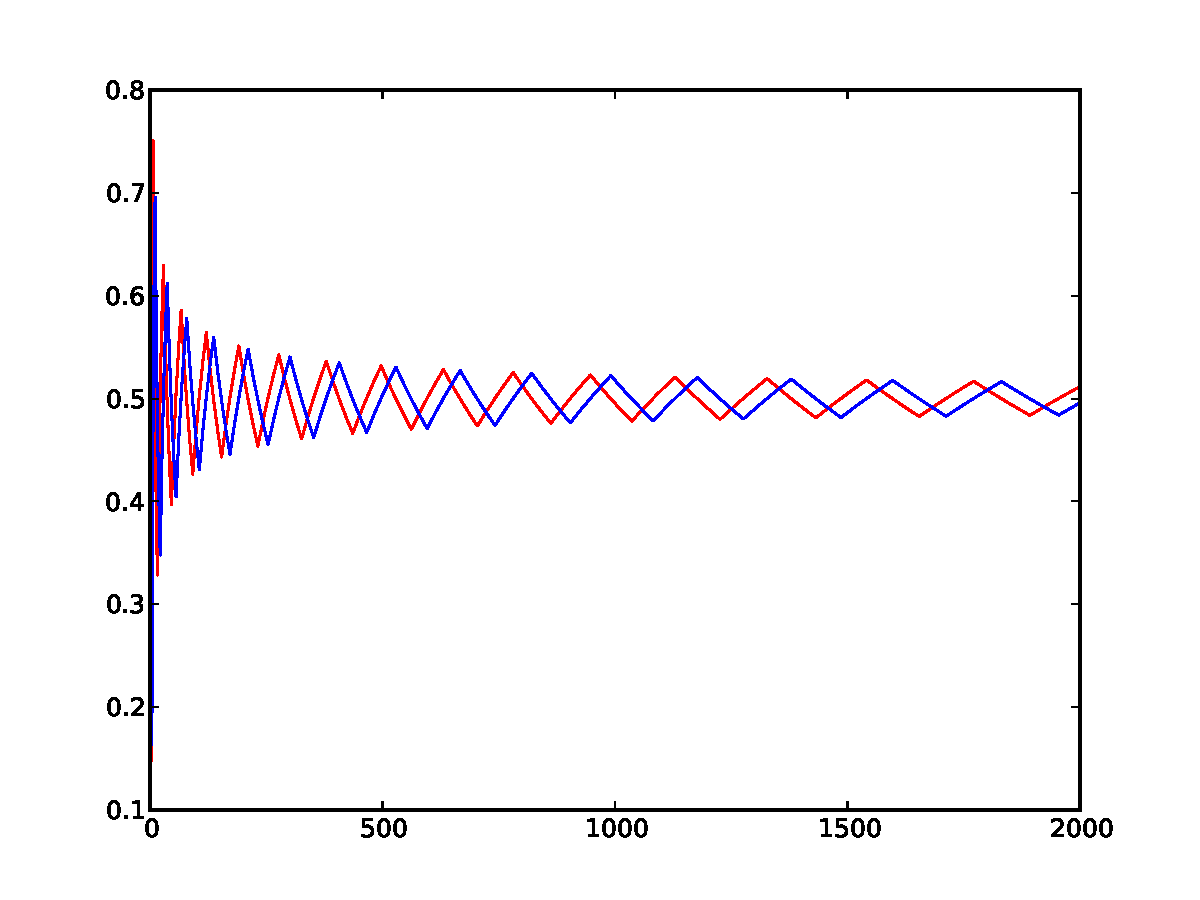
\includegraphics[width=7.5cm]{fictitious.pdf}
 \caption{$x_0(t)$と$x_1(t)$の推移}
 \label{fig:fictitious plot}
 
\end{figure}
\begin{itemize}\setlength{\parskip}{0.5em}
\item
回数を重ねるほどどちらも$0.5$に近づく
\end{itemize}
\end{frame}




\begin{frame}
\frametitle{ヒストグラム}
\begin{figure}
 \centering
 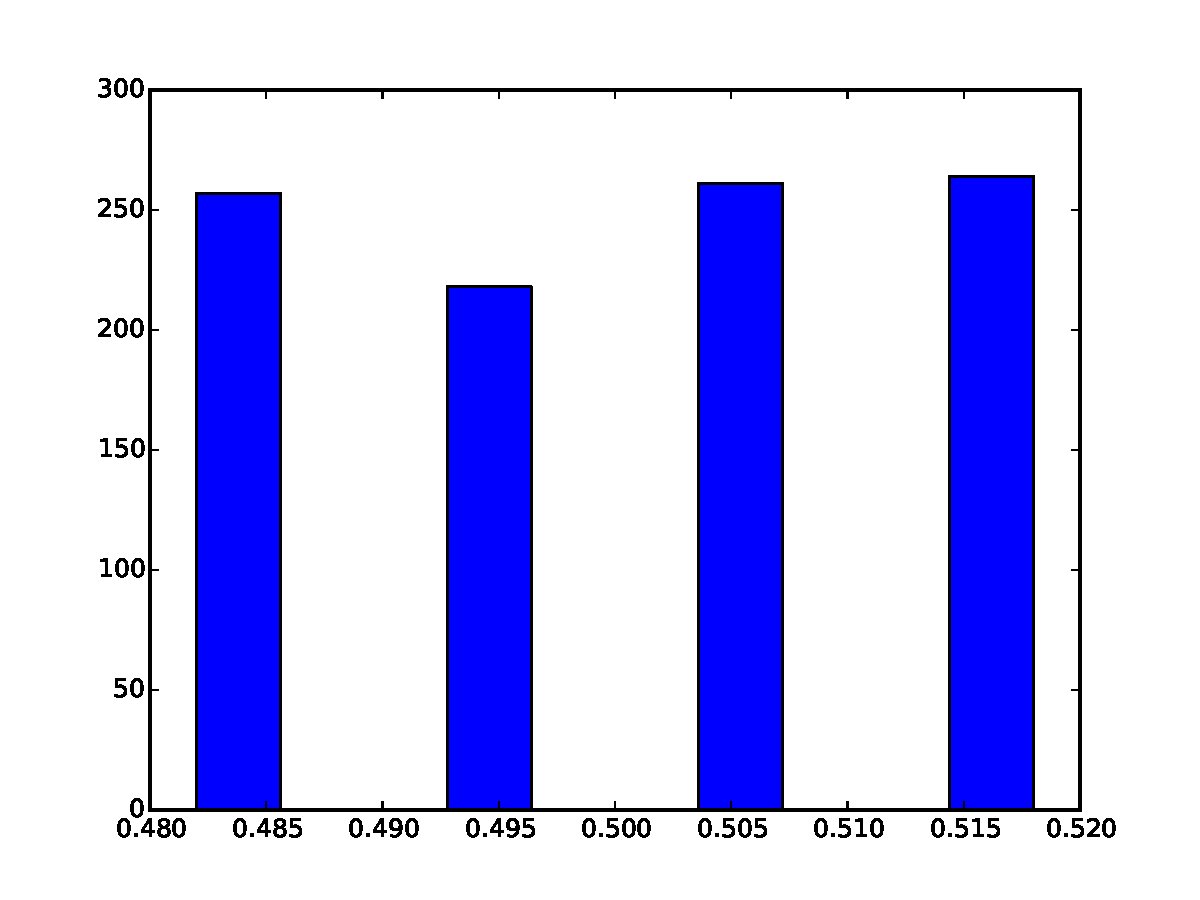
\includegraphics[width=8.5cm]{fictitious_hist.pdf}
 \caption{1000回Matching Penniesゲームを行う試行を1000回繰り返したときの最終期の信念の頻度分布}
 \label{fig:histgram}
\end{figure}
\end{frame}


\begin{frame}
\frametitle{まとめ}
\begin{itemize}\setlength{\parskip}{0.5em}


\item
今後の課題
 \begin{itemize}\setlength{\parskip}{0.5em}
 \item
classを定義するのがまだ自分のなかで理解しきれていない
 \item
利得行列をプレイヤー0と1それぞれ入力しないといけない状態のままになっている

 \end{itemize}
\item
\LaTeX は少しずつですが慣れてきました

もう少しスピードアップをはかりたいです



\end{itemize}
\end{frame}






\end{document}
